O método de Fibonacci é um método iterativo utilizado para a localização do mínimo de funções. Esse método utiliza um intervalo $ I_k $ = [a b], escolhemos então dois pontos simétricos em relação ao centro. Chamando $ x_1 $=a e $ x_4 $=b os pontos escolhidos serão $ x_2 $ e $ x_3 $. como pode ser visto na \ref{fig:ab}

\begin{figure}[h]
	\begin{center}
		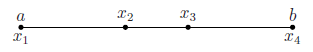
\includegraphics[width=8cm]{../fibonacci/intervalo_inicial.png}   
		\caption{Segmento de reta $ \overline{ab} $}
		\label{fig:ab}
	\end{center}
\end{figure}

O mecanismo de redução do intervalo é bem simples, usa-se o critério dos 2 pontos. Para determinar o próximo intervalo $ I_k+1 $ calcula-se o valor da função f em $ x_2 $ e $ x_3 $, resultando em $ f_2 $ e $ f_3 $. Se $ f_2 $ < $ f_3 $ então [$ x_1 $ $ x_3 $] será o novo intervalo (\ref{fig:x1x3}) e se $ f_2 $ > $ f_3 $, então retemos [$ x_2 $ $ x_4 $] (\ref{fig:x2x4}). No caso de igualdade entre $ f_2 $ e $ f_3 $ a escolha é indiferente. 

\begin{figure}[h]
	\begin{center}
		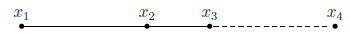
\includegraphics[width=8cm]{../fibonacci/x1x3.png}   
		\caption{Intervalo antigo e novo}
		\label{fig:x1x3}
	\end{center}
\end{figure}

\begin{figure}[h]
	\begin{center}
		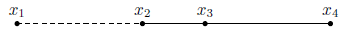
\includegraphics[width=8cm]{../fibonacci/x2x4.png}   
		\caption{Intervalo antigo e novo}
		\label{fig:x2x4}
	\end{center}
\end{figure}

Criamos então o novo intervalo $ I_k+1 $, caso ele seja:
\begin{itemize}
	\item [$ x_1 $ $ x_3 $] $\rightarrow$ $ x_1 $ permanece $ x_1 $, $ x_3 $ se torna o novo $ x_4 $, $ x_2 $ se torna o novo $ x_3 $ e um novo $ x_2 $ é colocado simetricamente ao novo $ x_3 $.
	\item [$ x_2 $ $ x_4 $] $\rightarrow$ $ x_4 $ permanece $ x_4 $, $ x_2 $ se torna o novo $ x_1 $, $ x_3 $ se torna o novo $ x_2 $ e um novo $ x_3 $ é colocado simetricamente ao novo $ x_2 $.
\end{itemize}

Só nos resta agora explicar como definir a escolha inicial de $ x_2 $ e $ x_3 $. Esses valores são escolhidos utilizando um fator 0,7 < $\alpha$ < 0,8, então algebricamente calculamos $ x_2  =  \alpha_1  x_1  + (1 -  \alpha_1 ) x_4 $ e $ x_3  = (1 -  \alpha_1 ) x_1  +  \alpha_1  x_4 $.
O valor de $\alpha$ é proveniente da fórmula utilizada para determinar o k-ésimo número da frequência de Fibonacci, portanto o método ganha esse nome.
Sendo k o número de reduções necessárias em determinado problema, podemos determinar o valor de $\alpha$ através de:
$\alpha = \dfrac{2}{1+\sqrt{5}} \times \dfrac{1-p^k}{1-p^{k+1}}$ onde $p=\dfrac{1-\sqrt{5}}{1+\sqrt{5}}$

Agora, com todas essas informações, podemos finalmente demonstrar o algoritmo que realmente será utilizado em sua forma computacional iterativa:
\textbf{Dados:}
\begin{itemize}
	\item $f:\mathbb{R}\rightarrow\mathbb{R}$, uma função suave e unimodal em
	\item $I_1=[ab]\subset\mathbb{R}$, intervalo enquadrante inicial
	\item $n\in\mathbb{Z}$ número desejado de reduções
	\item $k\in\mathbb{Z}$ índice de Fibonacci ($=n+1$)
\end{itemize}
\textbf{Objetivo:} Encontrar $I_n \subset I_1$ que enquadre um mínimo de $f$
\textbf{Operações:}
\begin{enumerate}
	\item $p=\dfrac{1-\sqrt{5}}{1+\sqrt{5}}$, $\alpha = \dfrac{2}{1+\sqrt{5}} \times \dfrac{1-p^k}{1-p^{k+1}}$
	\item $i=1$
	\item $x_1=a;\; x_4=b;\; L_{ini}=b-a;$
	\item $x_2=\alpha x_1+(1-\alpha)x_4;\; f_2=f(x_2)$
	\item $x_3=\alpha x_4 + (1 - \alpha)x_1;\; f_3 = f(x_3)$
	\item $ f_2 < f_3 $
	
	\begin{itemize}
		\item $a=x_1;\; b=x_3;\; L_{fin}=b-a;$
		\item $i=n \rightarrow I_n = [ab] \rightarrow FIM$
		\item $\alpha = \dfrac{(L_{ini}-L_{fin})}{L_{fin}};\; i=i+1$
		\item volta a 3.
	\end{itemize}
	

	\begin{itemize}
		\item $f_2 \geq f_3$
		\item $a=x_2;\; b=x_4;\; L_{fin}=b-a;$
		\item $i=n \rightarrow I_n=[ab] \rightarrow FIM$
		\item $\alpha = \dfrac{(L{ini}-L_{fin})}{L_{fin}};\; i=i+1$
		\item volta a 3.
	\end{itemize}
\end{enumerate}

Com o algoritmo de Fibonacci construído, foram testadas quatro funções para efeitos de comparação:

\begin{itemize}
	\item $ f_1(x) = 3x^2 + 20x - 8 $
	\item $ f_2(x) = xsin(x)cos(x) $
	\item $ f_3(x) = 5x $
	\item $ f_4(x) = -e^{-\mid x \mid} $
\end{itemize}

\newpage

Os resultados para a função $ f_1(x) $ foram:

\begin{figure}[h]
	\begin{center}
		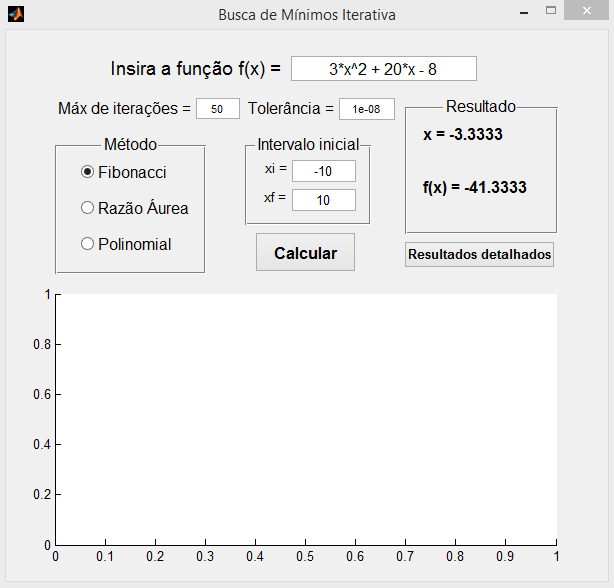
\includegraphics[width=13cm]{../fibonacci/f1_gui.png}   
		\caption{Janela de inicialização de $ f_1(x) $}
		\label{fig:fibonacci-f1-gui}
	\end{center}
\end{figure}

\begin{figure}[h!]
	\begin{center}
		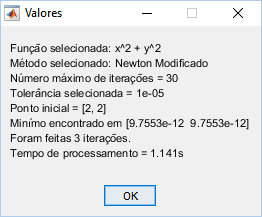
\includegraphics[width=6cm]{../fibonacci/f1_resultados.png}   
		\caption{Resultados detalhados de $ f_1(x) $}
		\label{fig:fibonacci-f1-resultados}
	\end{center}
\end{figure}

Os resultados para a função $ f_2(x) $ foram:

\begin{figure}[h]
	\begin{center}
		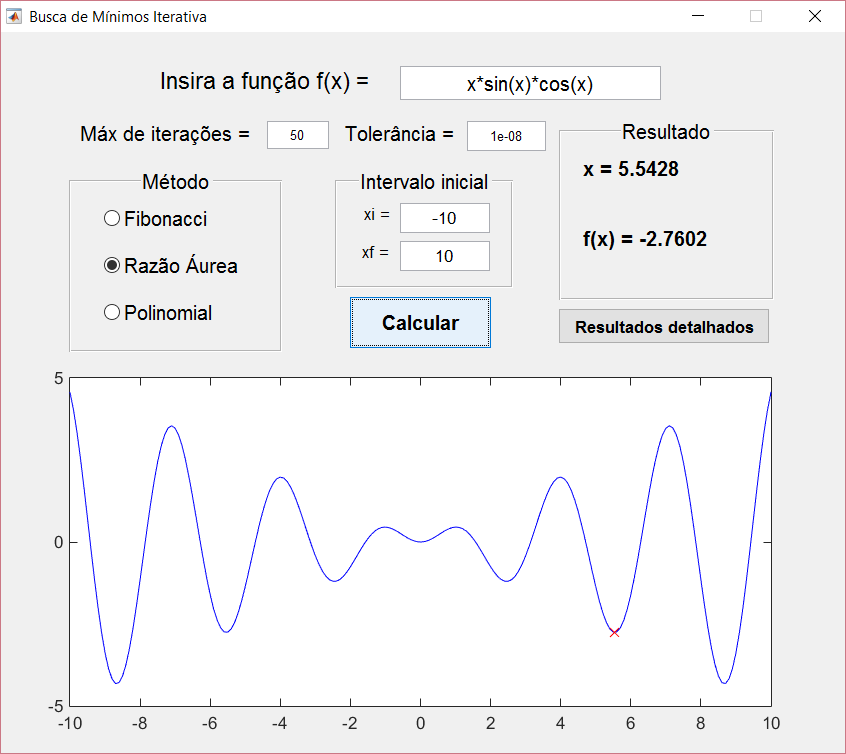
\includegraphics[width=13cm]{../fibonacci/f2_gui.png}   
		\caption{Janela de inicialização de $ f_2(x) $}
		\label{fig:fibonacci-f2-gui}
	\end{center}
\end{figure}

\begin{figure}[h!]
	\begin{center}
		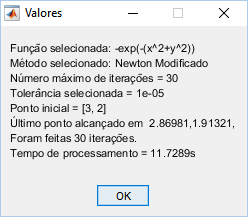
\includegraphics[width=6cm]{../fibonacci/f2_resultados.png}   
		\caption{Resultados detalhados de $ f_2(x) $}
		\label{fig:fibonacci-f2-resultados}
	\end{center}
\end{figure}

Os resultados para a função $ f_3(x) $ foram:

\begin{figure}[h]
	\begin{center}
		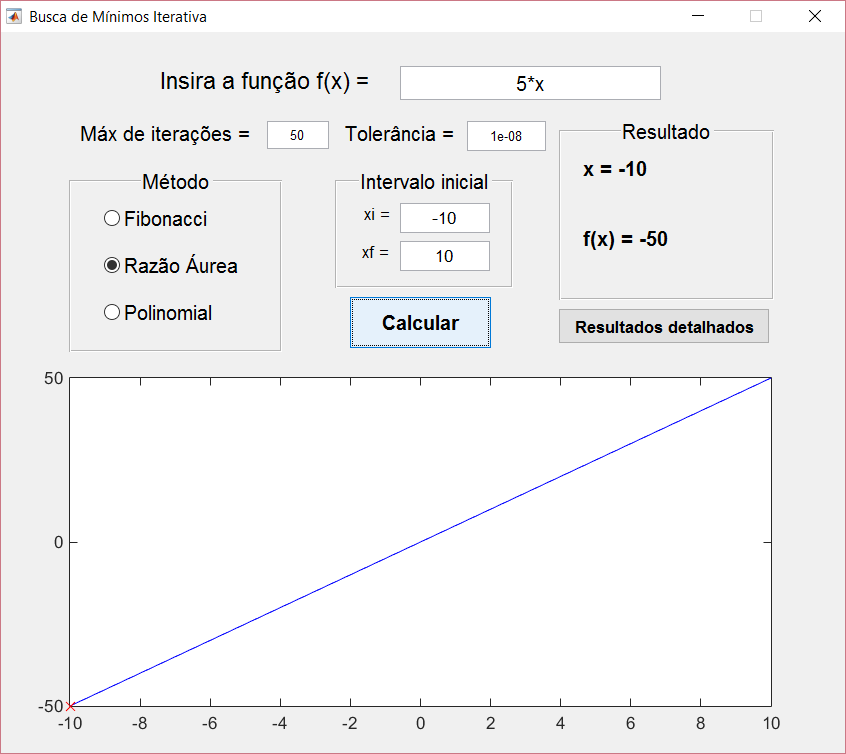
\includegraphics[width=13cm]{../fibonacci/f3_gui.png}   
		\caption{Janela de inicialização de $ f_3(x) $}
		\label{fig:fibonacci-f3-gui}
	\end{center}
\end{figure}

\begin{figure}[h!]
	\begin{center}
		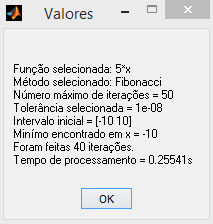
\includegraphics[width=6cm]{../fibonacci/f3_resultados.png}   
		\caption{Resultados detalhados de $ f_3(x) $}
		\label{fig:fibonacci-f3-resultados}
	\end{center}
\end{figure}

Os resultados para a função $ f_4(x) $ foram:

\begin{figure}[h]
	\begin{center}
		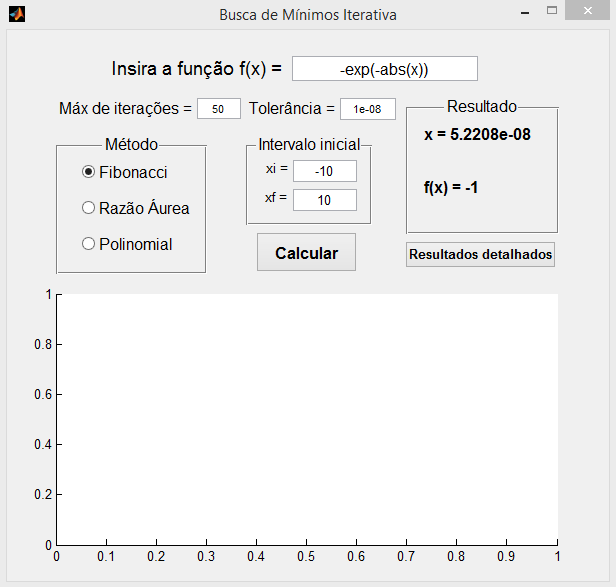
\includegraphics[width=13cm]{../aurea/f4_gui.png}   
		\caption{Janela de inicialização de $ f_4(x) $}
		\label{fig:fibonacci-f4-gui}
	\end{center}
\end{figure}

\begin{figure}[h!]
	\begin{center}
		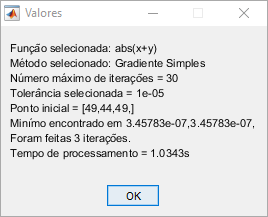
\includegraphics[width=6cm]{../aurea/f4_resultados.png}   
		\caption{Resultados detalhados de $ f_4(x) $}
		\label{fig:fibonacci-f4-resultados}
	\end{center}
\end{figure}
